\section{Εισαγωγή}
Στα πλαίσια της δεύτερης εργασίας του μαθήματος Advanced Machine Learning καλούμαστε να εφαρμόσουμε διάφορες τεχνικές σχετικές κυρίως με προβλήματα μάθησης από πολλαπλές ετικέτες (multi-label) και πολλαπλών παραδειγμάτων (multi-instance), καθώς επίσης και να εφαρμόσουμε την μέθοδο ενεργούς μάθησης (active learning) σε ένα δεδομένο πρόβλημα ταξινόμησης. 
Για την εφαρμογή όλων των παραπάνω, θα χρησιμοποιηθεί το σύνολο δεδομένων \emph{DeliciousMIL} όπως έχει δοθεί σχετική οδηγία στην εκφώνηση της εργασίας.

\subsection{Σύνολο Δεδομένων}
Το \emph{DeliciousMIL} είναι ένα σύνολο δεδομένων το οποίο δημιουργήθηκε από τους \cite{Soleimani} με στόχο να εξυπηρετήσει την έρευνα γύρω από προβλήματα ταξινόμησης πολλαπλών ετικετών και πολλαπλών παραδειγμάτων με κύριο αντικείμενο την ταξινόμηση κειμένου σε επίπεδο εγγράφων και προτάσεων.

Τα έγγραφα που περιέχονται στην εν λόγω συλλογή προέρχονται από το site delicious.com και συλλέχθηκαν την περίοδο του Ιουνίου 2008. Οι ετικέτες που αναγνωρίστηκαν είναι συνολικά 20 και περιγράφονται στον Πίνακα \ref{tab: labels}.

	\begin{table*}
	\centering
	\caption{Περιγραφή των Ετικετών}
	\label{tab: labels}
	\begin{tabular}{cccccccc}
		\hline
		\ttfamily index  & \ttfamily class & \ttfamily index  & \ttfamily class &
		\ttfamily index  & \ttfamily class & \ttfamily index  & \ttfamily class \\ \hline
		1 & reference	& 6	& web		&	11	&	style  & 16 & politics   \\ \hline
		2 & design		& 7	& java		&	12	&	language  & 17 & religion  \\ \hline
		3 & programming & 8	& writing	&	13	&	books  & 18 & science  \\ \hline
		4 & internet	& 9	& English	&	14	&	education  & 19 & history  \\ \hline
		5 & computer	& 10& grammar	&	15	&	philosophy  & 20 & culture \\ \hline
	\end{tabular}
\end{table*}

Το μέγεθος του συνόλου των δεδομένων είναι 12234 έγγραφα τα οποία έχουν χωριστεί σε δύο υποσύνολα: 
	\begin{itemize}
		\item Εκπαίδευσης με 8251 έγγραφα
		\item Επαλήθευσης με 3983 έγγραφα
	\end{itemize}


Η συχνότητα εμφάνισης της κάθε κλάσης φαίνεται στην Εικόνα \ref{fig: label_distribution}

\begin{figure}
	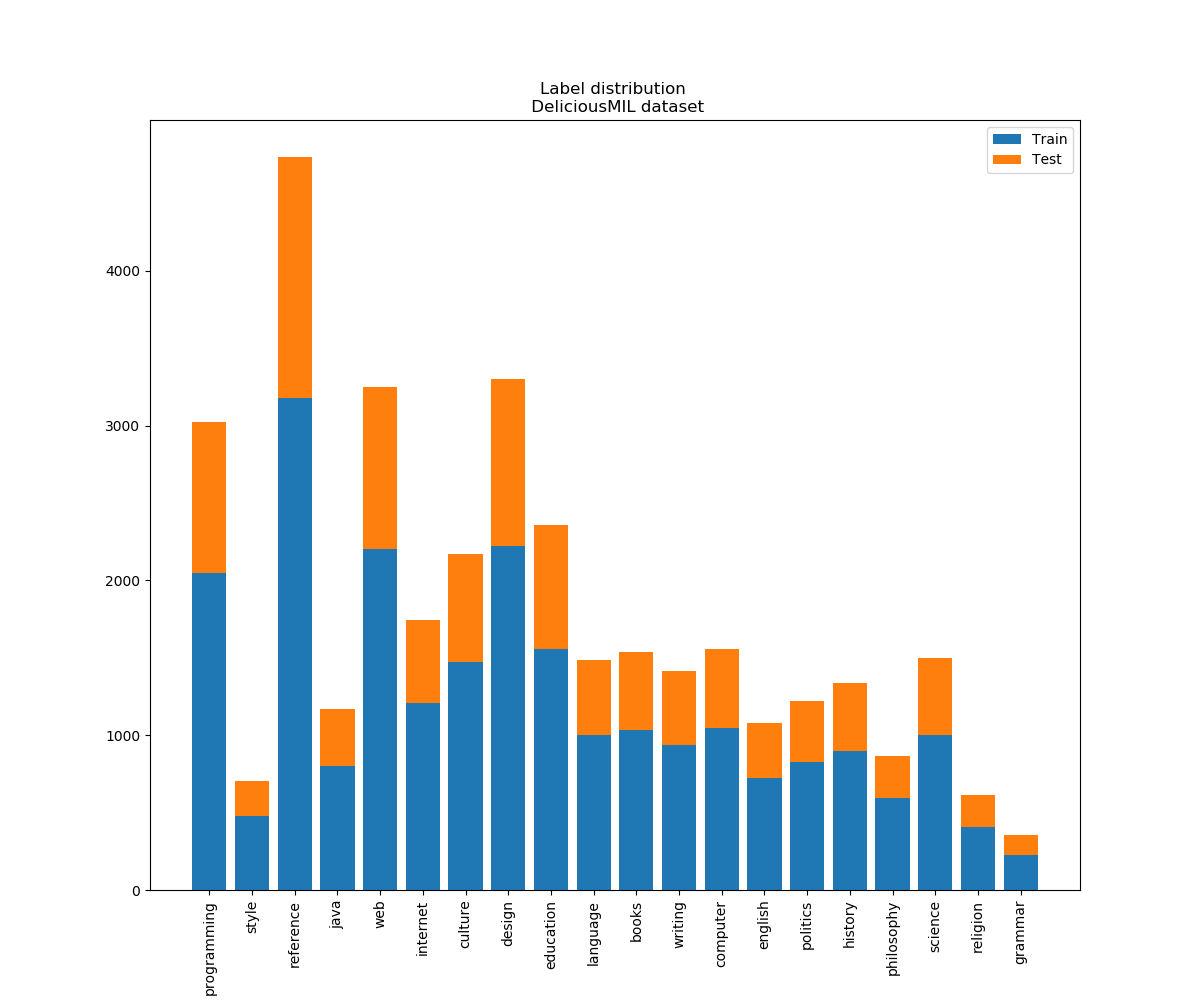
\includegraphics[width=\textwidth,center]{label_distribution.png}
	\caption{Πλήθος εμφανίσεων της κάθε ετικέτας στο Train και στο Test σετ των δεδομένων.}
	\label{fig: label_distribution}
\end{figure}


Το DeliciousMIL είναι ελεύθερα διαθέσιμο στο αποθετήριο του UC Irvine Machine Learning Repository \footnote{https://archive.ics.uci.edu/ml/machine-learning-databases/00418/}


\section{Μέρος Α}
Για το πρώτο μέρος της εργασίας ζητήθηκε η εφαρμογή μία μεθόδου μάθησης από δεδομένα πολλαπλών ετικετών. Για την υλοποίηση του παραπάνω χρησιμοποιήθηκε η μέθοδος Classifier Chain και συγκεκριμένα εφαρμόσθηκε μία ensemble εκδοχή με vote averaging. Για την αξιολόγηση των αποτελεσμάτων επιλέχθηκε η μετρική \emph{macro-averaged F-measure}. Στην θέση του βασικού αλγορίθμου για την εφαρμογή της μεθόδου χρησιμοποιήθηκαν οι Naive Bayes, Decision Tree \& SVM with gaussian kernel. 

\subsection{Προεπεξεργασία δεδομένων}
Για την υλοποίηση των παραπάνω ήταν απαραίτητη η προ-επεξεργασία των δεδομένων προκειμένου να είναι έτοιμα προς χρήση. Αρχικά, από κάθε έγγραφο αφαιρέθηκε η πληροφορία για το πόσες λέξεις υπάρχουν ανά έγγραφο και ανά πρόταση. Σε δεύτερο στάδιο από την απλή καταγραφή των λέξεων που δινόταν, δημιουργήθηκε ένα διάνυσμα με το σύνολο των λέξεων και την καταγραφή των εμφανίσεων της κάθε λέξης ανά έγγραφο. Για την συνέχεια της εργασίας επιλέχθηκε η χρήση της συγκεκριμένης μορφοποίησης των δεδομένων. Η κατανομή της συχνόητητας εμφάνισης της κάθε λέξης φαίνεται στο Σχήμα \ref{fig: word_distribution}

\begin{figure}
	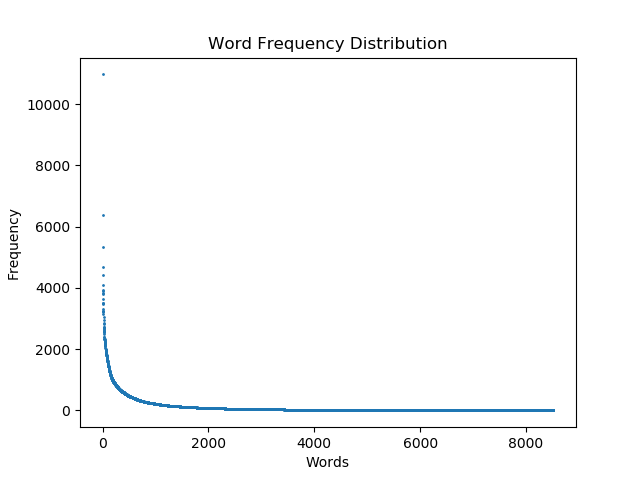
\includegraphics[width=0.75\textwidth,center]{word_distribution.png}
	\caption{Αριθμός εμφανίσεων των λέξεων που βρίσκονται στο σύνολο της συλλογής. Η εκτύπωση είναι σε αύξοντα αριθμό εμφανίσεων.}
	\label{fig: word_distribution}
\end{figure}


 
\subsection{Πειραματική Διαδικασία}


Αφού ολοκληρώθηκε η προ-επεξεργασία των δεδομένων, και για την εφαρμογή της μεθόδου classifier chain ήταν απαραίτητη η αντιμετώπιση του προβλήματος σε δυαδικό επίπεδο. Για την ικανοποίηση της συγκεκριμένης απαίτησης επιλέχθηκε η μέθοδος OneVsRest. Αφού προέκυψε το μοντέλο με τα συγκεκριμένα χαρακτηριστικά, εφαρμόσθηκε η μέθοδος Classifier Chain όπου ορίστηκαν 20 chains και η F-measure macro ως μετρική αξιολόγησης. Για το σύνολο της παραπάνω διαδικασίας επιλέχθηκε η εφαρμογή διαφόρων αλγορίθμων ταξινόμησης. Συγκεκριμένα εφαρμόσθηκαν οι SVM with gaussian kernel, Decision Tree \& Naive Bayes.

Για την υλοποίηση του πρώτου μέρους χρησιμοποιήθηκε η python 2.7 και η βιβλιοθήκη scikit-learn. Επιπλέον, χρησιμοποιήθηκαν τροποποιημένα τα παραδείγματα που υπάρχουν στην βιβλιοθήκη για την εφαρμογή των μεθόδων και την εκτύπωση των αποτελεσμάτων.
Πλέον της μεθόδου Classifier Chain, υπολογίστηκαν αποτελέσματα και με την OneVSRest μέθοδο.

\subsection{Αποτελέσματα}

Στα Σχήματα \ref{fig: CC_NB}, \ref{fig: CC_DT} \& \ref{fig: CC_SVM} φαίνονται οι αποδόσεις της εφαρμογής του classifier chain με διαφορετικό αλγόριθμο ταξινόμησης κάθε φορά.



\begin{figure}
	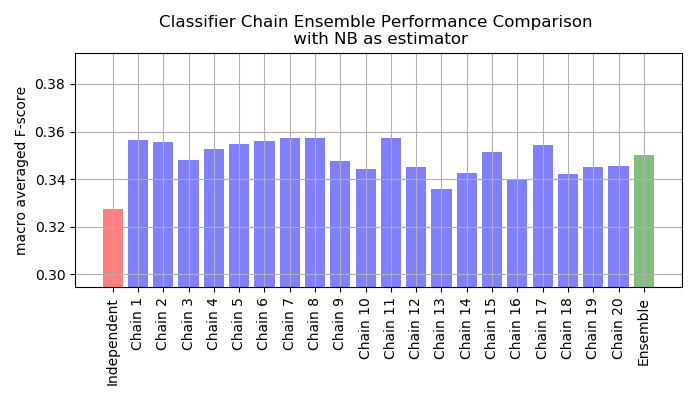
\includegraphics[width=\textwidth,center]{CC_NB.png}
	\caption{F score Macro Average για όλα τα chains στον Classifier Chain. Η πρώτη μπάρα (Independent) μας δείχνει την απόδοση ταξινομητή πριν την εφαρμογή του Classifier Chain ενώ η τελευταία μας δείχνει το αποτέλεσμα της ensemble διαδικασίας. Ο αλγόριθμος ταξινόμησης είναι ο Naive Bayes}
	\label{fig: CC_NB}
\end{figure}

\begin{figure}
	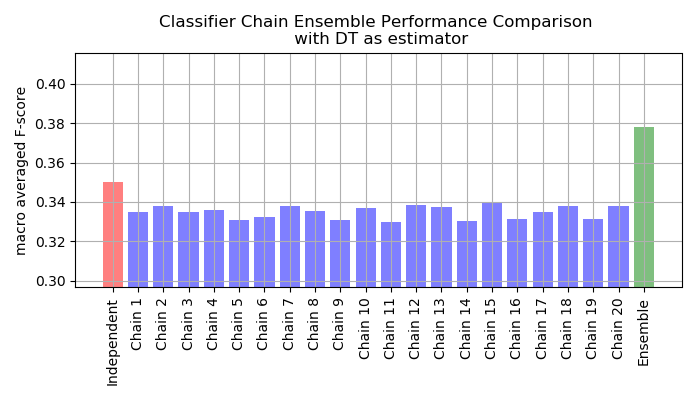
\includegraphics[width=\textwidth,center]{CC_DT.png}
	\caption{F-score Macro Average για όλα τα chains στον Classifier Chain. Η πρώτη μπάρα (Independent) μας δείχνει την απόδοση ταξινομητή πριν την εφαρμογή του Classifier Chain ενώ η τελευταία μας δείχνει το αποτέλεσμα της ensemble διαδικασίας. Ο αλγόριθμος ταξινόμησης είναι ένα Δέντρο Απόφασης.}
	\label{fig: CC_DT}
\end{figure}

\begin{figure}
	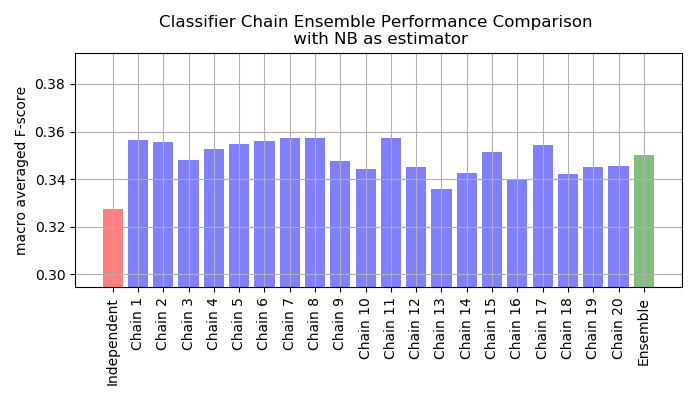
\includegraphics[width=\textwidth,center]{CC_NB.png}
	\caption{F-score Macro Average για όλα τα chains στον Classifier Chain. Η πρώτη μπάρα (Independent) μας δείχνει την απόδοση ταξινομητή πριν την εφαρμογή του Classifier Chain ενώ η τελευταία μας δείχνει το αποτέλεσμα της ensemble διαδικασίας. Ο αλγόριθμος ταξινόμησης είναι ένα SVM with rbf kernel.}
	\label{fig: CC_SVM}
\end{figure}


Στα Σχήματα \ref{fig: 1vsR_NB}, \ref{fig: 1vsR_DT} \& \ref{fig: 1vsR_SVM} φαίνονται οι αποδόσεις μετά την εφαρμογή της μεθόδου OneVsRest για κάθε ετικέτα με διαφορετικό αλγόριθμο ταξινόμησης κάθε φορά.


\begin{figure}
	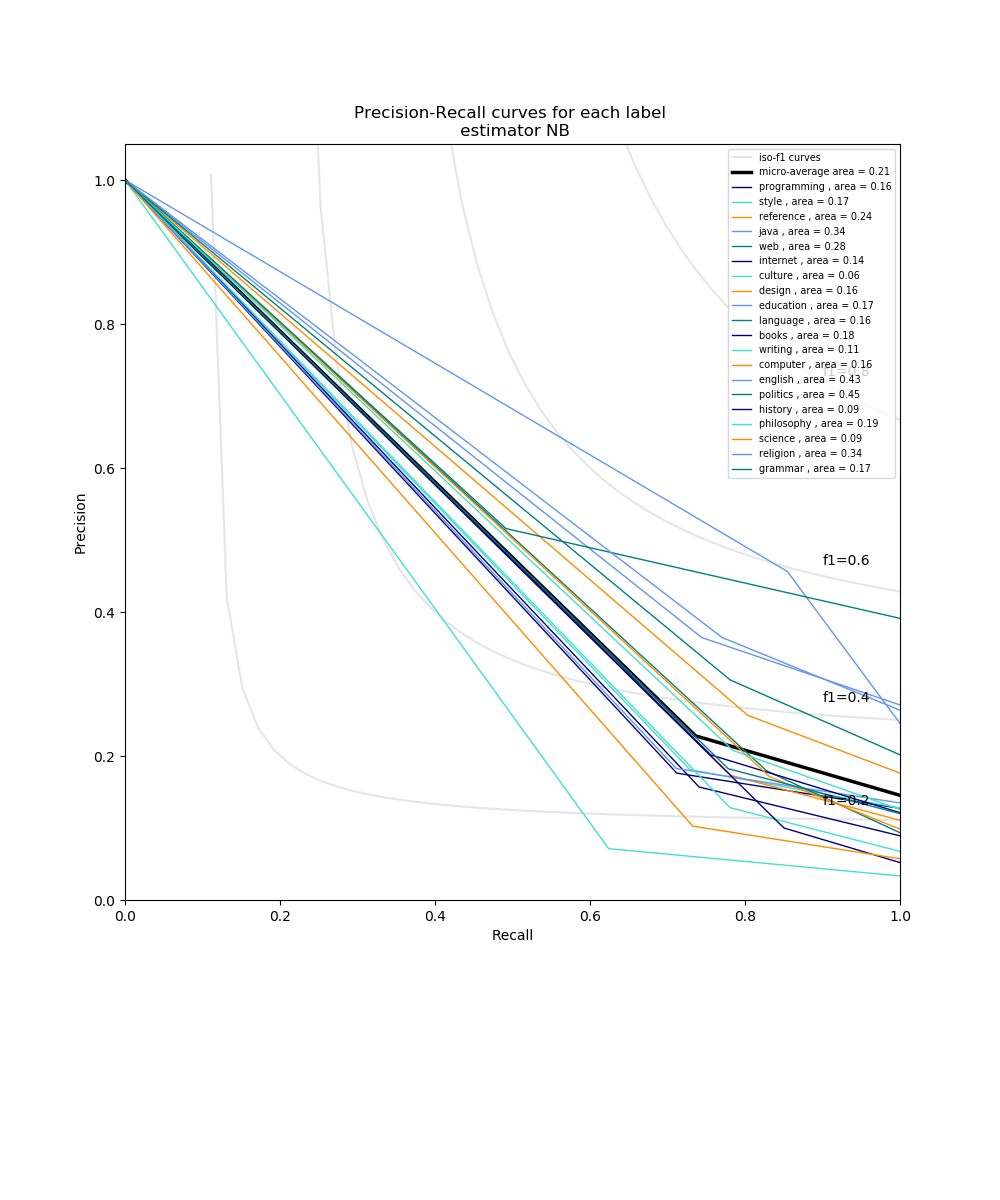
\includegraphics[width=0.8\textwidth,center]{1vsR_NB.png}
	\caption{micro F-score  για όλες τις ετικέτες μετά την εφαρμογή της OneVSRest μεθόδου με αλγόριθμο ταξινόμησης τον Naive Bayes.}
	\label{fig: 1vsR_NB}
\end{figure}


\begin{figure}
	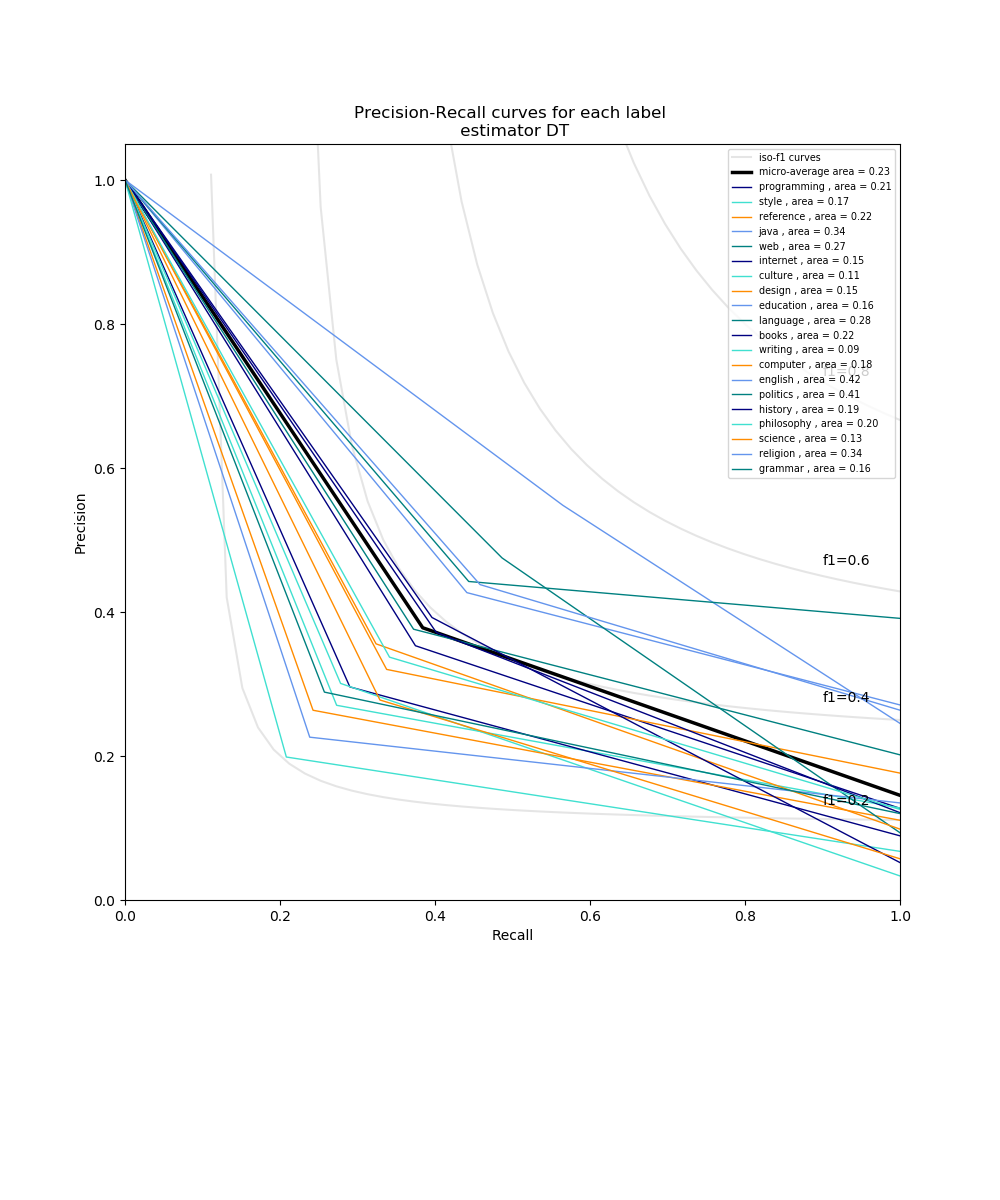
\includegraphics[width=0.8\textwidth,center]{1vsR_DT.png}
	\caption{micro F-score  για όλες τις ετικέτες μετά την εφαρμογή της OneVSRest μεθόδου με αλγόριθμο ταξινόμησης ένα Δέντρο Απόφασης.}
	\label{fig: 1vsR_DT}
\end{figure}


\begin{figure}
	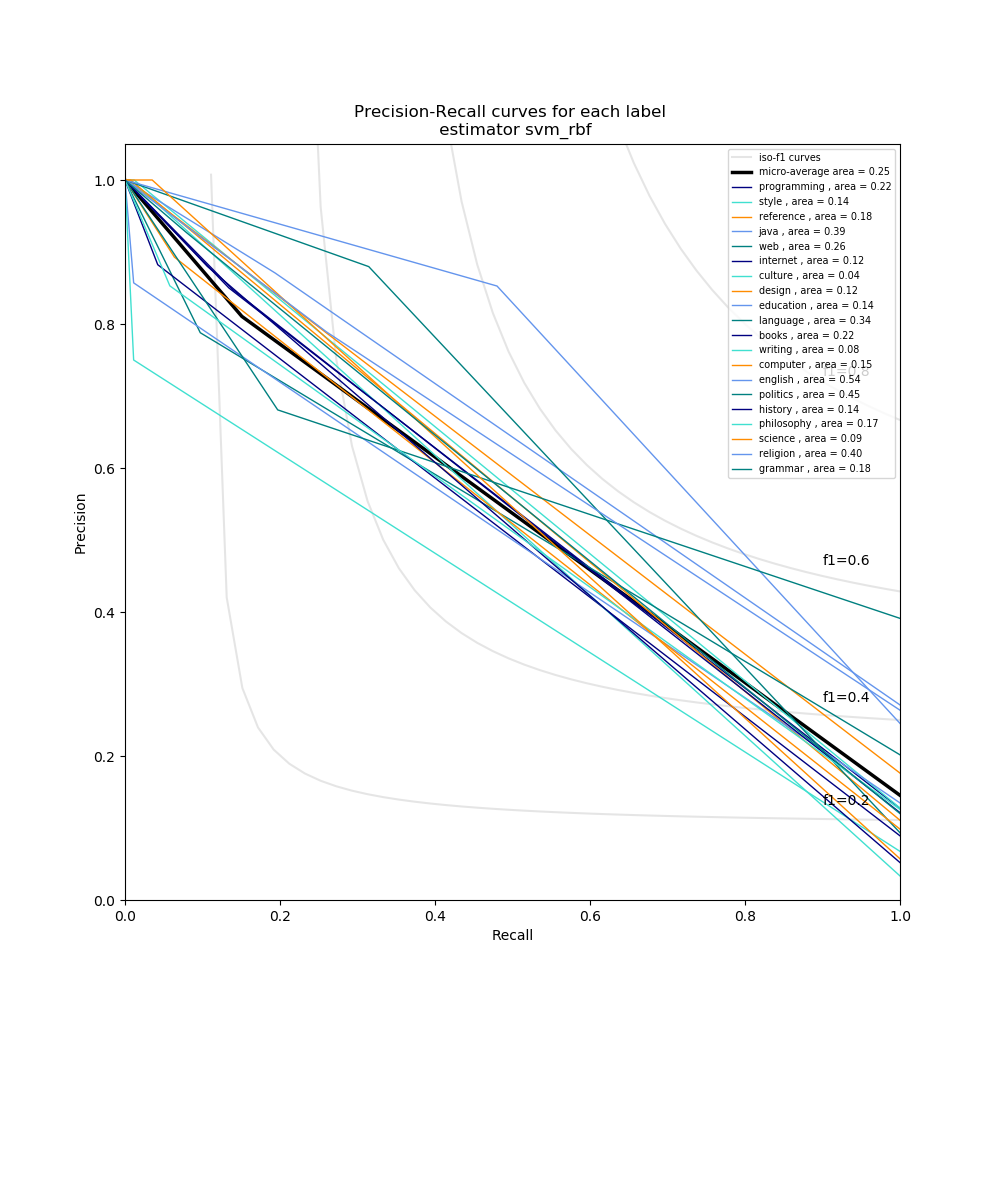
\includegraphics[width=0.8\textwidth,center]{1vsR_SVM.png}
	\caption{micro F-score  για όλες τις ετικέτες μετά την εφαρμογή της OneVSRest μεθόδου με αλγόριθμο ταξινόμησης ένα SVM.}
	\label{fig: 1vsR_SVM}
\end{figure}
\newpage
\section{Μέρος Β}

Στο δεύτερο μέρος της εργασίας ζητούμενο η επίλυση ενός προβλήματος μάθησης από σάκους περιπτώσεων. Για την απλοποίηση του προβλήματος κληθήκαμε να δουλέψουμε με την συχνότερη κλάση έτσι ώστε να μετατραπεί σε πρόβλημα δυαδικής ταξινόμησης. Σύμφωνα με το Σχήμα \ref{fig: label_distribution} η κλάση με τις περισσότερες εμφανίσεις στο σύνολο δεδομένων είναι η \emph{reference}. Για την συγκεκριμένη υλοποίηση αποφασίσθηκε ο μετασχηματισμός του προβλήματος σε ένα κλασσικό πρόβλημα μηχανικής μάθησης. 


\subsection{Μετασχηματισμός Δεδομένων}

Για τον μετασχηματισμό των δεδομένων, χρησιμοποιήθηκε η "κλασσική υπόθεση" (classical assumption) ενώ "σάκος" θεωρήθηκε το κάθε έγγραφο και "περίπτωση" η κάθε πρόταση.
Στη συνέχεια, για λόγους επάρκειας υπολογιστικών πόρων, περιορίστικε το μέγεθος του train set σε 3000 έγγραφα και το test set σε 1000. Σε αυτά τα σύνολα δεδομένων εφαρμόσθηκε ο παραπάνω μετασχηματισμός και κατόπιν ο αλγόριθμος 20-means. Μετά την εφαρμογή του 20-means και τον εκ νέου μετασχηματισμό της αναπαράστασης των δεδομένων, το πρόβλημα ήταν δυνατό να επιλυθεί με την εφαρμογή ενός αλγορίθμου δυαδικής ταξινόμησης. Για αυτό το μέρος χρησιμοποιήθηκε ο SVM linear, ο Naive Bayes και o Decision Tree.

\subsection{Αποτέλεσματα}

%[[538  45]
%[375  43]]

%[[571  12]
%[400  18]]

%[[299 284]
%[224 194]]


\begin{table}[]
	\centering
	\caption{Αποτελέσματα για την ταξινόμηση με σάκους περιπτώσεων για την κλάση "reference"}
	\label{tab: bags of instances}
	\begin{tabular}{|c|c|c|c||c|c||c|c|}
		\hline
		\multicolumn{2}{|c|}{{\color[HTML]{343434} }}                   & \multicolumn{6}{c|}{\textbf{true}}                                            \\ \cline{3-8} 
		\multicolumn{2}{|c|}{{\color[HTML]{343434} }}                   & \multicolumn{2}{c||}{\textbf{NB}} & \multicolumn{2}{c||}{\textbf{SVM}} & \multicolumn{2}{c|}{\textbf{DT}}\\ \cline{3-8} 
		\multicolumn{2}{|c|}{\multirow{-3}{*}{{\color[HTML]{343434} }}} & \textbf{0}          & \textbf{1}          & \textbf{0}      & \textbf{1}  & \textbf{0}      & \textbf{1}    \\ \hline
		& \textbf{0}         & 538                 & 45                  & 571             & 12 &299 &284              \\ \cline{2-8} 
		\multirow{-2}{*}{\textbf{predict}}         & \textbf{1}         & 375                 & 43                  & 400             & 18 &224 &194               \\ \hline
	\end{tabular}
\end{table}


\begin{figure}
%	\centering{}
	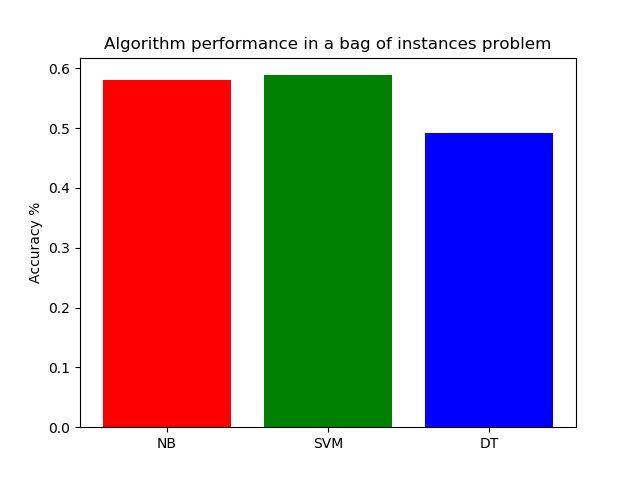
\includegraphics[width=.6\textwidth,center]{20means.png} %[width=0.6\textwidth]
	\caption{Αποτελέσματα ταξινόμησης για την περίπτωση της ταξινόμησης με σάκους περιπτώσεων.}
	\label{fig: bag of instances}
\end{figure}

Τα αποτελέσματα της παραπάνω διαδικασίας περιγράφονται στον Πίνακα \ref{tab: bags of instances}. Στην πρώτη περίπτωση ο ταξινομητής πέτυχε Acc= 0.58, στην δεύτερη πέτυχε Acc= 0.59 ενώ στην τρίτη Acc=0.49. Παρατηρώντας τον πίνακα σύγχυσης ( Πίνακας \ref{tab: bags of instances} ) μπορεί κανείς να συμπεράνει εύκολα ότι τα αποτελέσματά μας δεν είναι ιδιαίτερα καλά. Είναι πολύ πιθανό να έχουμε χάσει πληροφορία στην αρχική προσέγγιση που κάναμε σε σχέση με την αναπαράσταση των λέξεων με bag of words και αυτό να μας έχει οδηγήσει εδώ.

\newpage
\section{Μέρος Γ}
Στο τρίτο και τελευταίο μέρος της εργασίας, κληθήκαμε να δουλέψουμε στο πρόβλημα της ενεργούς μάθησης. Για την υλοποίηση του συγκεκριμένου μέρους, χρησιμοποιήσαμε μόνο το test set του DeliciousMIL dataset. Το πρόβλημα από πολλαπλών ετικετών μετασχηματίστηκε σε δυαδικής ταξινόμησης καθώς ασχοληθήκαμε μόνο με την σπανιότερη κλάση (grammar) όπως φαίνεται από την κατανομή των κλάσεων στo Σχήμα \ref{fig: label_distribution}. 

\subsection{Περιγραφή Πειράματος}

Όπως αναφέρθηκε και παραπάνω, για την υλοποίηση του συγκεκριμένου μέρους της εργασίας χρησιμοποιήθηκε μόνο το test set του αρχικού συνόλου δεδομένων, το οποίο χωρίστηκε σε δύο επι μέρους σύνολα, το "unlabeled pool set" και το test set. Για την αρχικοποίηση του πειράματος δημιουργήθηκε ένα πρώτο train set από το "unlabeled pool set" το οποίο αποτελείται από 8 παραδείγματα, 4 της κλάσης 0 και 4 της κλάσης 1. 

Για την εφαρμογή του αλγορίθμου uncertainty sampling ακολουθήθηκε η παρακάτω διαδικασία:
Με δεδομένο το αρχικό σύνολο εκπαίδευσης που περιγράφηκε παραπάνω, εκπαιδεύτηκε ο αλγόριθμος SVM. Από το μοντέλο που προέκυψε υπολογίστηκαν οι πιθανότητες για κάθε παράδειγμα του υπολειπόμενου unlabeled pool set. Σε αυτές τις τιμές εφαρμόσθηκε ο τύπος $ 𝑥∗=argmin_𝑥|𝑃(𝑦_1|𝑥)−0.5|$ και επιλέχθηκε το επόμενο παράδειγμα το οποίο πρόκειται να δοθεί για annotation. Αφού έγινε ο σχολιασμός του συγκεκριμένου παραδείγματος, αυτό τοποθετήθηκε στο train set και αφαιρέθηκε από το unlabeled pool set. Με το train set εκπαιδεύτηκε εκ νέου ο αλγόριθμος SVM και συνεχίστηκε η διαδικασία για συνολικά δέκα επαναλήψεις. 

%\begin{algorithm}
%	\SetKwInOut{Train}{Input}
%	\SetKwInOut{Output}{Output}
%	
%	\underline{Process}
%	\Input{Two nonnegative integers $a$ and $b$}
%	\Output{$\gcd(a,b)$}
%	\eIf{$b=0$}
%	{
%		return $a$\;
%	}
%	{
%		return Euclid$(b,a\mod b)$\;
%	}
%	\caption{Active learning with uncertainty sampling}
%\end{algorithm}
 


\subsection{Αποτελέσματα}

Για την αξιολόγηση της διαδικασίας του active learning with uncertainty sampling επιλέχθηκε η εκτύπωση καμπυλών μάθησης σε σύγκριση με την τυχαία επιλογή δειγμάτων. Τα αποτελέσματα φαίνονται στο Σχήμα \ref{fig: Active Learning Curves}


\begin{figure}
%	\centering{example-image}
	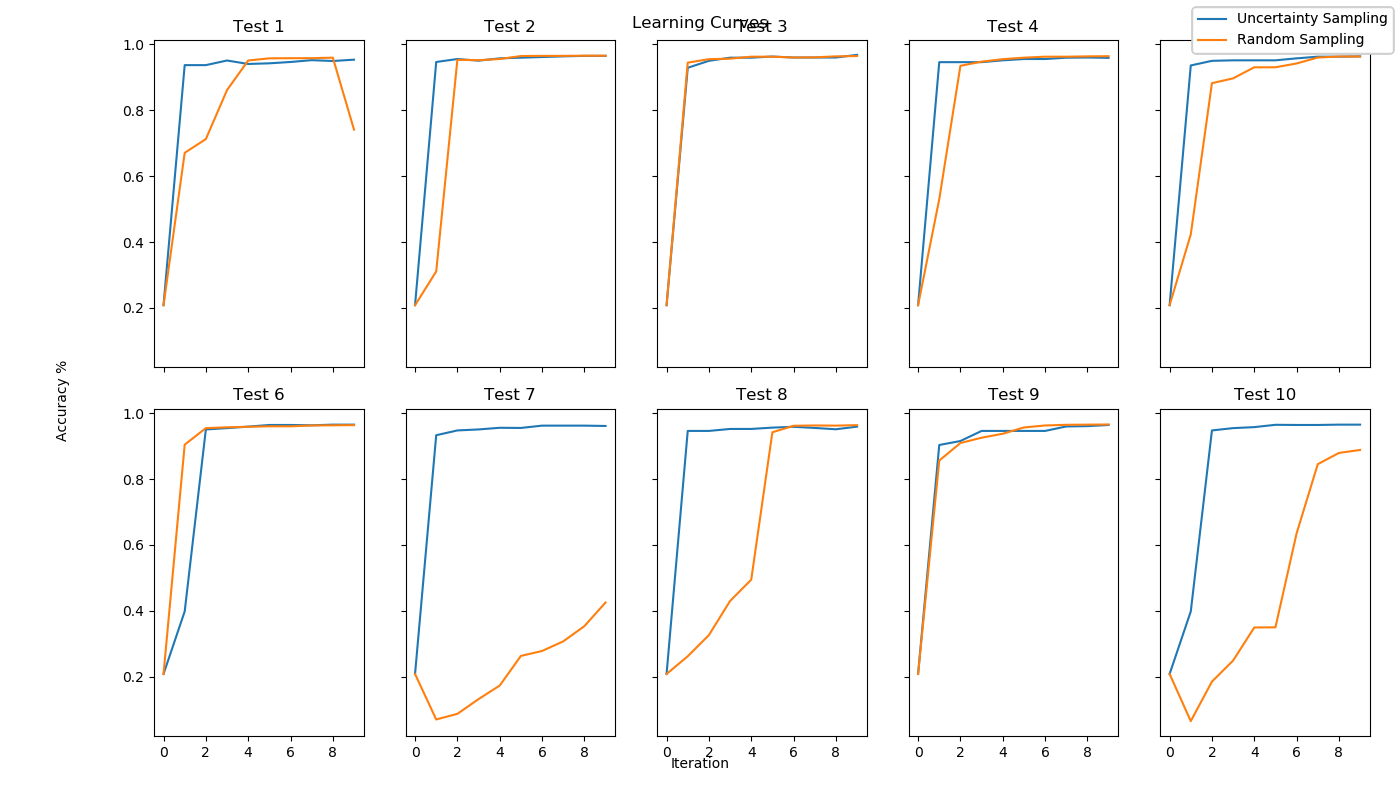
\includegraphics[width=.95\textwidth,left]{ALearningCurves.png} %[width=0.6\textwidth]
	\caption{Καμπύλες μάθησης i. για την διαδικασία Active Learning with Uncertainty sampling, ii. για Active Learning with Random Sampling. Για κάθε περίπτωση υπήρξαν 10 επαναλήψεις. Για το ίδιο dataset έγιναν 10 επαναλήψεις στο σύνολο.}
	\label{fig: Active Learning Curves}
\end{figure}


Παρατηρώντας το Σχήμα \ref{fig: Active Learning Curves} μπορούμε να συμπεράνουμε ότι τις περισσότερες φορές η μέθοδος active learning with uncertainty sampling οδηγεί γρηγορότερα και με μεγαλύτερη ασφάλεια στην αύξηση της ακρίβειας του ταξινομητή μας. Επιπλέον, είναι φανερό ότι τις φορές που υπερτερεί η random sampling είναι καθαρά θέμα τύχης. Μία ακόμα παρατήρηση που παρουσιάζει ενδιαφέρον είναι η σταθερότητα απόδοσης του μοντέλου με την μέθοδο uncertainty sampling σε αντίθεση με την random sampling κάτι που φαίνεται από την συμπεριφορά σε όλα τα πειράματα καθώς επίσης και ότι δεν επιρρεάζεται από τον αριθμό των επαναλήψεων σε αντίθεση με την random sampling, που για παράδειγμα στο πείραμα 1 στην δέκατη επανάληψη η ακρίβεια πρόβλεψης μειώνεται σημαντικά.


\section{Τεχνικά}

Στην ενότητα αυτή γίνεται μία σύνοψη των εργαλείων που για την εκπόνηση της εργασίας.
Όλα τα μέρη αυτής της εργασίας υλοποιήθηκαν σε Python 2.7 με την χρήση της βιβλιοθήκης scikit-learn \citep{scikit-learn}. Για ορισμένες διαδικασίες χρησιμοποιήθηκε κώδικας που βρίσκεται στα παραδείγματα της εν λόγω βιβλιοθήκης. Το σύνολο της εργασίας (κώδικας, σύνολα δεδομένων καθώς και τα αποτελέσματα μαζί με τα .tex αρχεία βρίσκονται στο https://github.com/ggravanis/AdvancedML . \\
Τα αρχεία κώδικα που αφορούν την δεύτερη εργασία είναι τα part[21-22-23].py. Στους φακέλους results/part[21-22-23] υπάρχουν επιπλέον αποτελέσματα από αυτά που βρίσκονται στο παρόν, ενώ στον φάκελο assignment2 βρίσκονται όλα τα αρχεία του τεύχους.
